\documentclass{article}
\usepackage{graphicx}
\usepackage{amsmath}     %数学宏包
\usepackage{amssymb}
\usepackage{mathtools}   %用来打<=号
\usepackage{indentfirst} %设置段首缩进宏包
\usepackage{paralist,multicol}
\usepackage{diagbox} %画斜表头

\usepackage{longtable}%跨页表格
\usepackage{array}   %使用表格环境tabular编辑表格
\renewcommand\arraystretch{1.5} \arraycolsep=0.8pt

\newcommand{\tab}{\makebox[2em][l]{}}   %段首缩进
\newcommand{\rea}[1]{$^{\left[ {#1} \right]}$}    %文内引用
\newcommand{\reb}[1]{${\left[ {\, #1\, } \right]}$\;\:}     %文末引用
\newcommand{\diff}{\mathrm{d}}   %打出微分的d
\setlength{\parindent}{0pt}   %设置段首不缩进


\usepackage[nocap]{ctexcap}   %设置字号用
\CTEXsetup[format={\heiti \zihao{4}}]{section}    %一级标题四号黑体
\CTEXsetup[format={\bf\heiti\zihao{5}}]{subsection}    %二级标题五号黑体
\setmainfont{Times New Roman} %阿拉伯数字为新罗马字体

\usepackage[paperheight=20cm,paperwidth=16cm,text={12cm,16.2cm}]{geometry}
\raggedcolumns %版心底部可以不对齐

\begin{document}


%题目**********************************************************

   \title{\heiti\zihao{3}5-stage-pipeline-cpu}
   \date{}
   \maketitle \vspace{-4em}



%功能汇总*****************************************************

   {\centering\section {功能汇总}}

   \subsection{目前进度}
   \begin{flushleft}
   \tab 写了一个32位5段流水的cpu,目前已实现register的内部上推功能,
   但memory的内部上推和cpu停止还没做。
   \end{flushleft}

   \subsection{文件命名}
   \begin{flushleft}
   \tab 设计文件中器件的命名按照《Computer organization and design》
   中的方式命名。\\
   \mbox{} \hfill{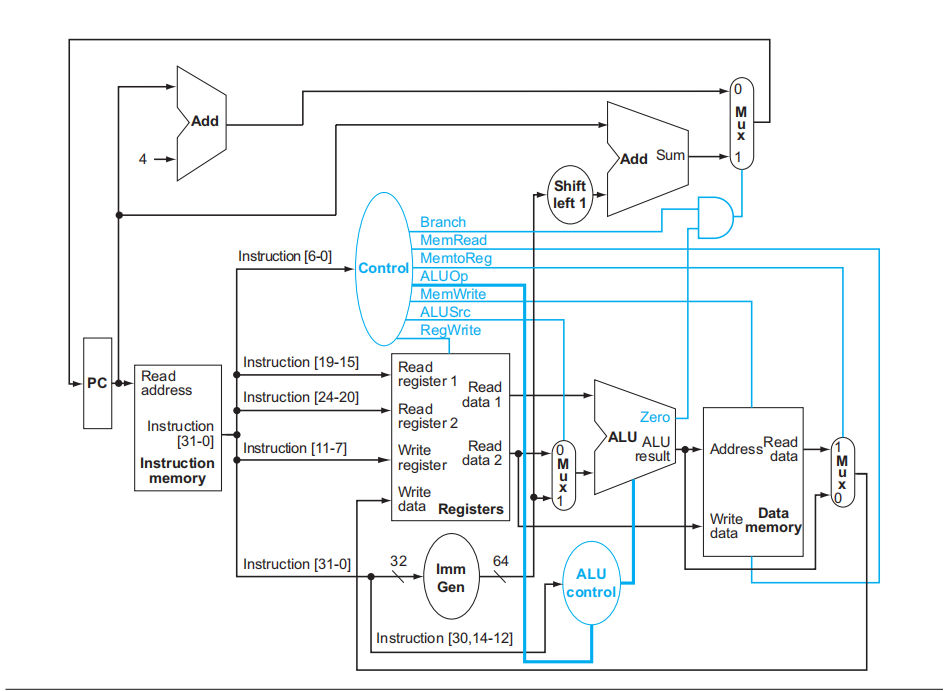
\includegraphics[scale=0.5]{1.png}}\hfill \mbox{}\\
   \end{flushleft}

   \subsection{实现函数}
   \begin{flushleft}
   \tab 该代码实现了以下20个函数:\\
   \mbox{} \hfill{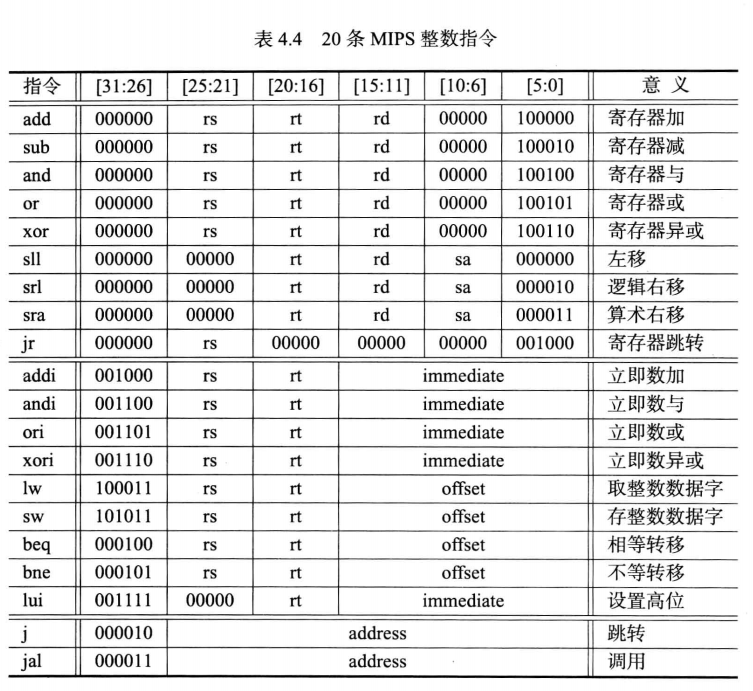
\includegraphics[scale=0.7]{2.png}}\hfill \mbox{}\\
   \end{flushleft}

   \subsection{结构图}
   \begin{flushleft}
   \tab 该cpu的结构图如下:\\
   \mbox{} \hfill{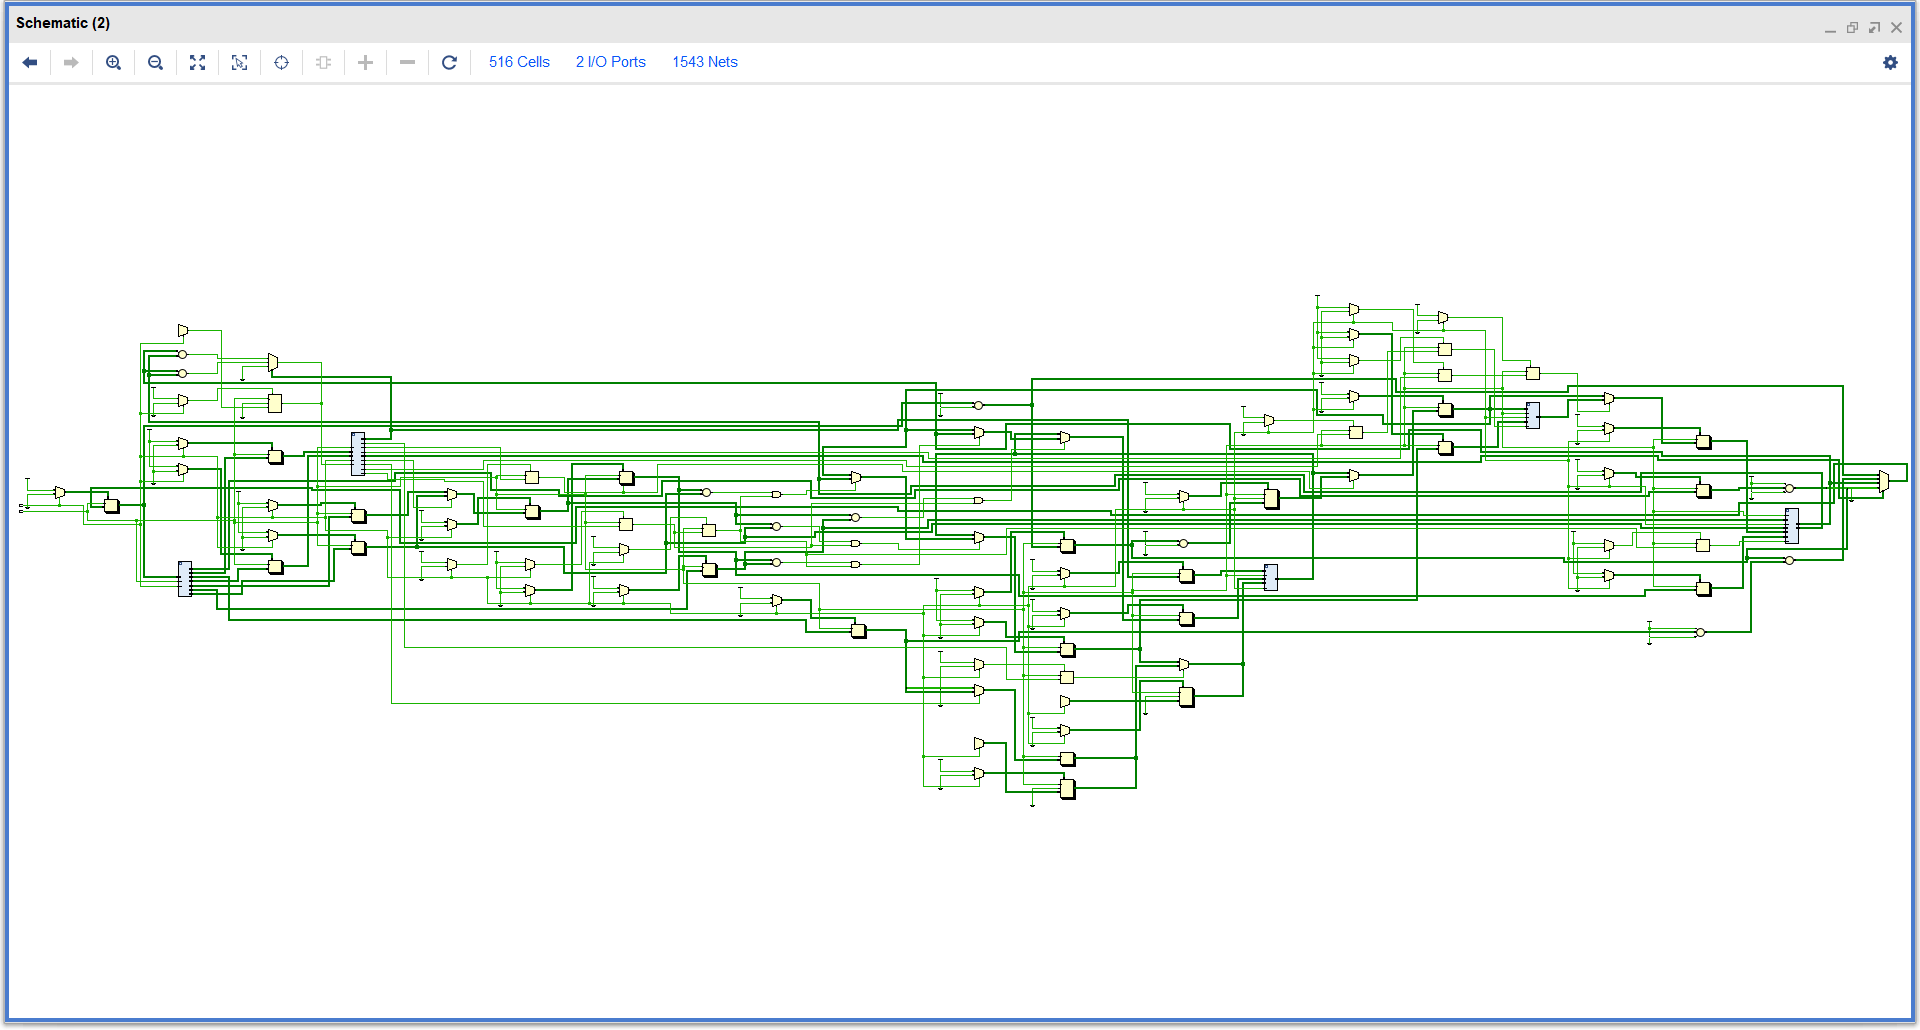
\includegraphics[scale=0.3]{11.png}}\hfill \mbox{}\\
   \end{flushleft}

%操作方法*****************************************************

{\centering\section {操作方法}}

   \subsection{代码写入}
   \begin{flushleft}
   \tab 在cpu运行前需要向instruction memory中写入cpu的软件代码,
   本模型采用了python模拟向instruction memory写入代码的过程。\\
   \tab 操作步骤如下:\\
   \tab 1.打开“指令转换”文件夹中的"decode.py"\\
   \mbox{} \hfill{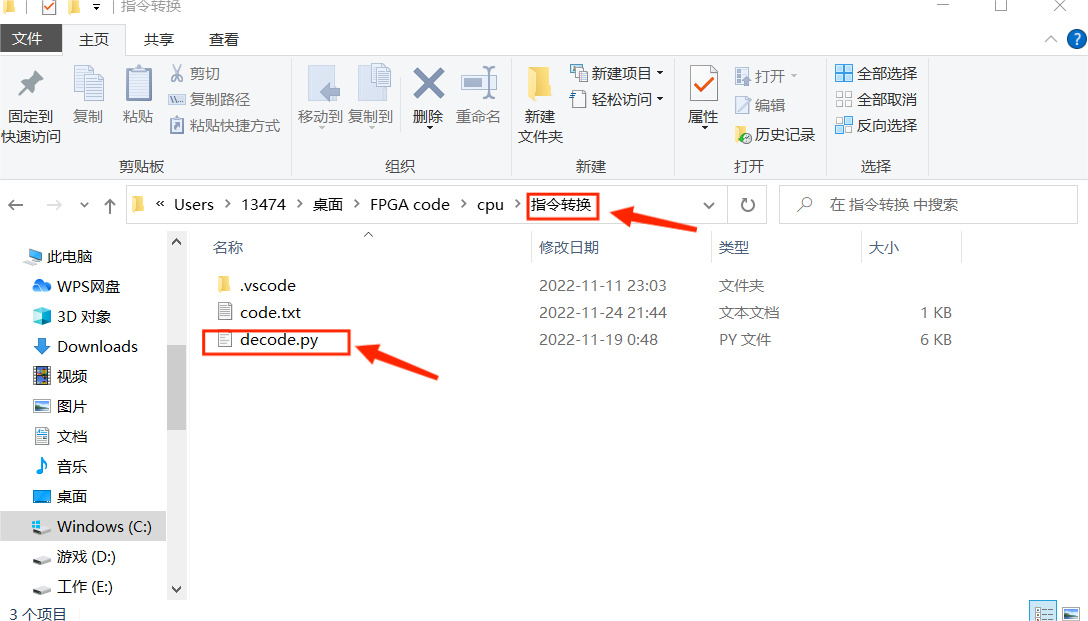
\includegraphics[scale=0.3]{3.png}}\hfill \mbox{}\\
   \tab 2.打开"decode.py"后,在debug模式下运行(直接运行好像会导致数据存不进文件),
   直接输入想要的代码即可。注意,要加入变量(如x1,x2,x3),应使用load函数,
   所有的变量都需要用load函数定义。\\
   \mbox{} \hfill{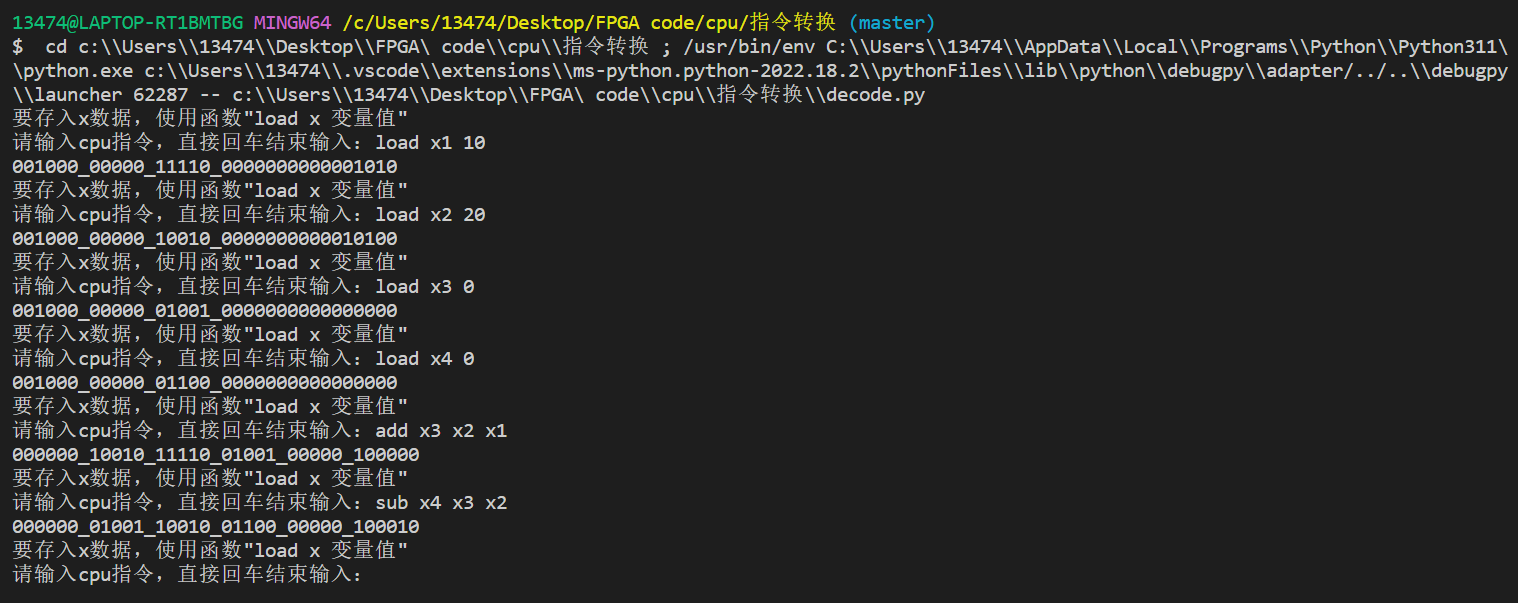
\includegraphics[scale=0.4]{4.png}}\hfill \mbox{}\\
   \tab 检查一下数据是否载入,打开"code.txt",即可看到刚刚生成的代码:\\
   \mbox{} \hfill{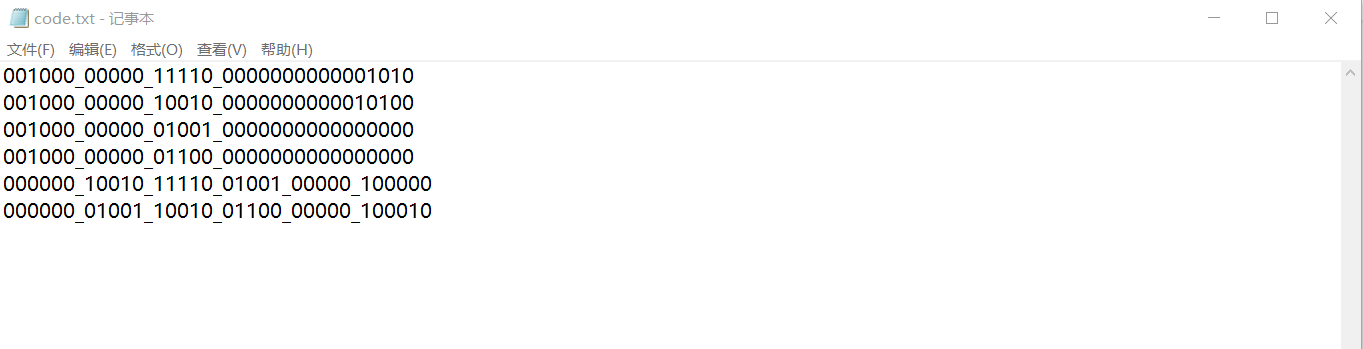
\includegraphics[scale=0.4]{5.png}}\hfill \mbox{}\\
   \tab 3.打开"design"文件夹的"instruction\_memory.v",用复制粘贴的形式
   将刚刚生成的代码输入对应区域即可。(尝试过\$readmemb,但好像加载不进去)\\
   \mbox{} \hfill{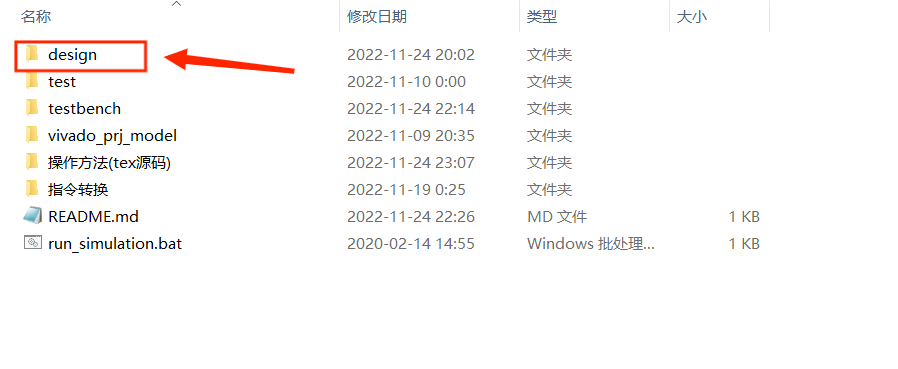
\includegraphics[scale=0.4]{6.png}}\hfill \mbox{}\\
   \mbox{} \hfill{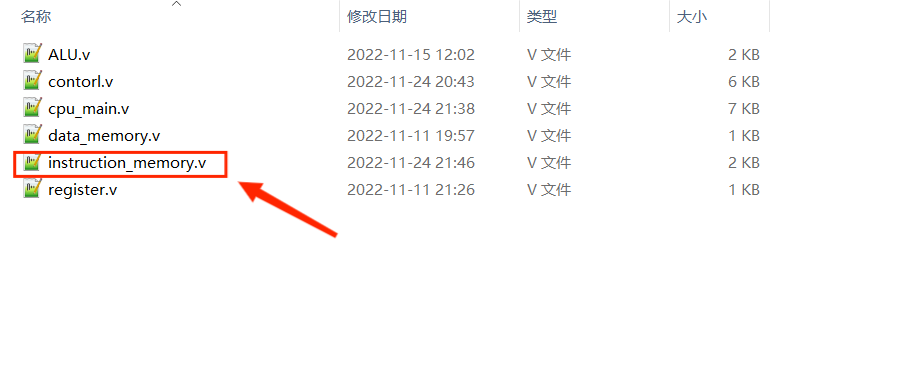
\includegraphics[scale=0.4]{7.png}}\hfill \mbox{}\\
   \mbox{} \hfill{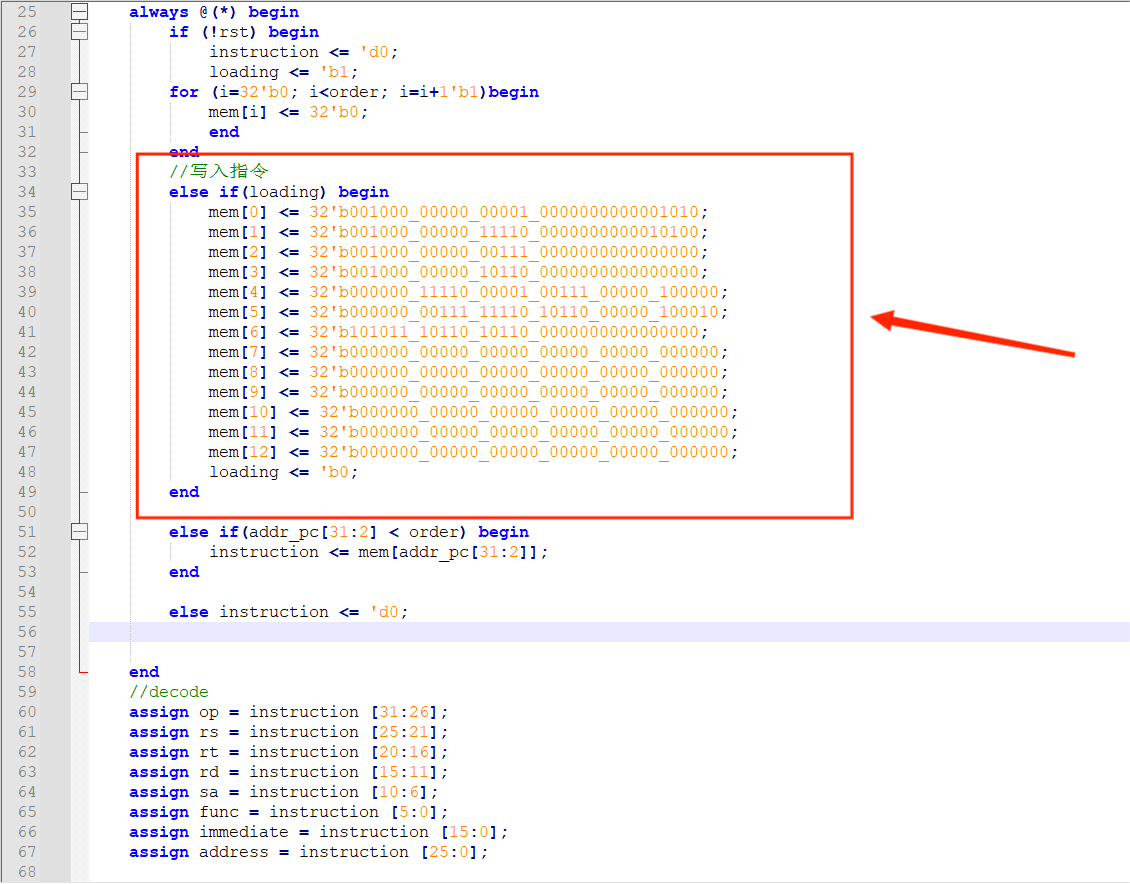
\includegraphics[scale=0.3]{8.png}}\hfill \mbox{}\\
   \tab 4.打开"run\_simulation.bat",按"1"运行即可。\\
   \mbox{} \hfill{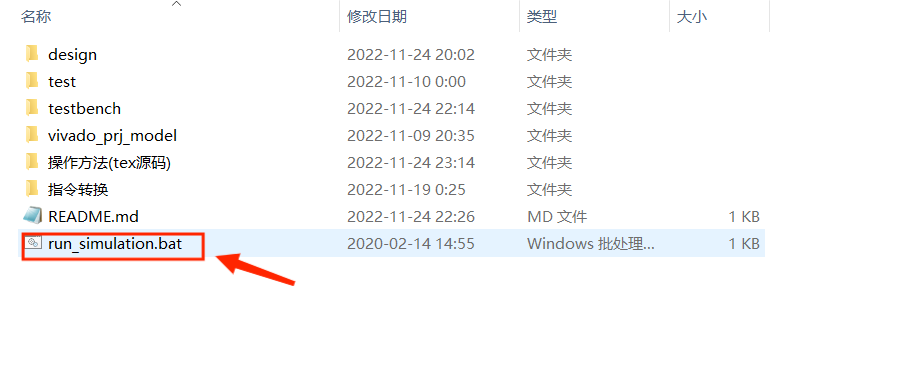
\includegraphics[scale=0.4]{9.png}}\hfill \mbox{}\\
   \tab 仿真开始后记得在'test'那里把想要的参数加进去。点击'RUN-ALL'开始运行就行。\\
   \mbox{} \hfill{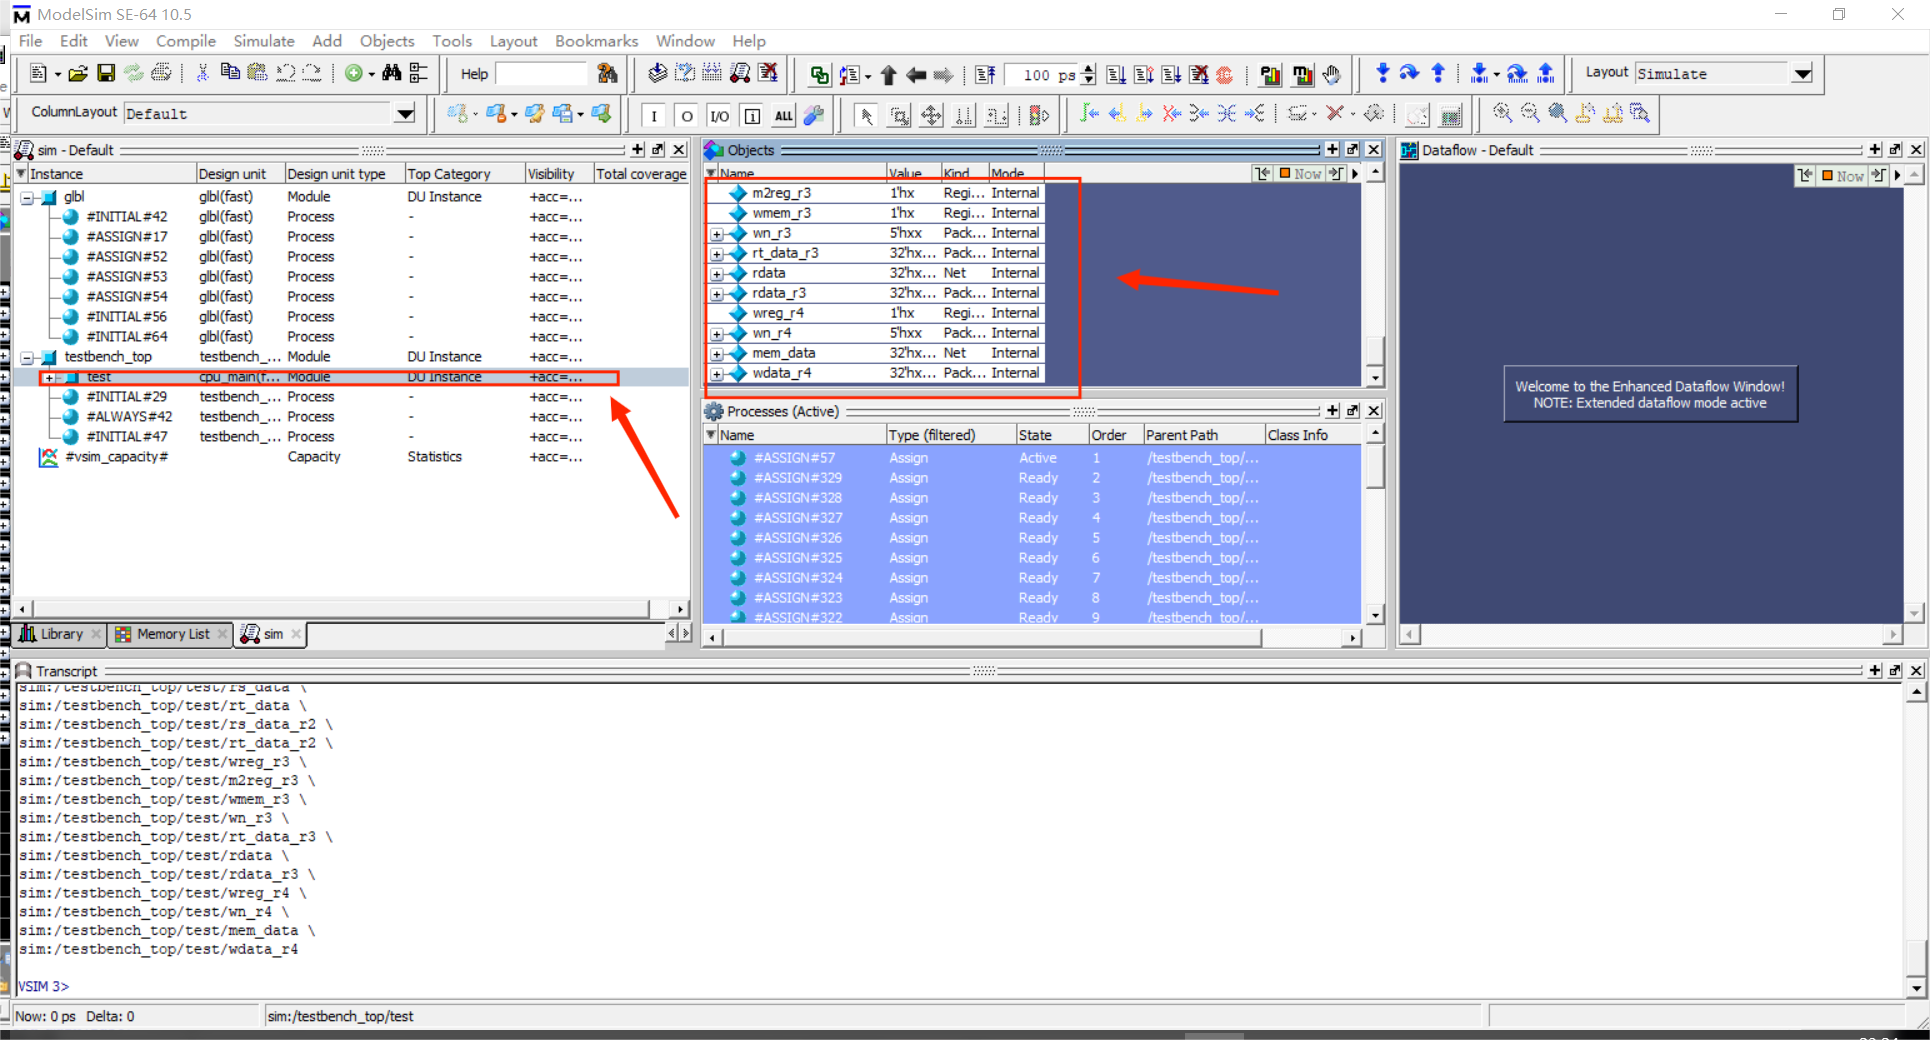
\includegraphics[scale=0.2]{10.png}}\hfill \mbox{}\\

   \end{flushleft}

%个人感想*****************************************************

{\centering\section {个人感想}}

\subsection{项目经历}
\begin{flushleft}
\tab 这个cpu现在已经做了一个多月,从10月初开始搞的。9月的时候我连verilog是啥都
不知道,搞了两个多月可以搞出一个能跑的cpu还是很高兴的。(虽然搞的不咋滴)\\
\tab 本来可以搞的更快一点的,但是考试还是有一点多,然后又要学英语,又要给实验室
画一些PCB,每天弄这个的时间不是很多,每天大概有两个小时吧。\\
\tab 9月份的时候学了一下啥叫verilog,写了几个小程序就开始搞这个了,
还是有一点难的,一开始找资料整了挺久。\\
\tab 后面有空的话会慢慢完善这个东西,不过期末考又差不多到了,不知道有没有空搞。
\end{flushleft}



          
\end{document}